% Ubah judul dan label berikut sesuai dengan yang diinginkan.

% % Ubah paragraf-paragraf pada bagian ini sesuai dengan yang diinginkan.

% % Contoh input beberapa gambar pada halaman.
% \begin{figure*}
%   \centering
%   \subfloat[Hasil A]{\includegraphics[width=.4\textwidth]{example-image-a}
%     \label{fig:hasila}}
%   \hfil
%   \subfloat[Hasil B]{\includegraphics[width=.4\textwidth]{example-image-b}
%     \label{fig:hasilb}}
%   \caption{Contoh input beberapa gambar.}
%   \label{fig:hasil}
% \end{figure*}

% \lipsum[16-18]

% % Contoh input potongan kode dari file.
% \lstinputlisting[
%   language=Python,
%   caption={Program perhitungan bilangan prima.},
%   label={lst:bilanganprima}
% ]{program/bilangan-prima.py}

% \lipsum[19-20]

% Update the title and label below as desired.
\section{Results and Discussion}
\label{sec:resultsanddiscussion}

% Update the paragraphs in this section as desired.

% % Example of inserting multiple images on a page.
% \begin{figure*}
%     \centering
%     \subfloat[Result A]{\includegraphics[width=.4\textwidth]{example-image-a}
%         \label{fig:resulta}}
%     \hfil
%     \subfloat[Result B]{\includegraphics[width=.4\textwidth]{example-image-b}
%         \label{fig:resultb}}
%     \caption{Example of inserting multiple images.}
%     \label{fig:result}
% \end{figure*}

% \lipsum[16-18]

% % Example of including a code snippet from a file.
% \lstinputlisting[
%     language=Python,
%     caption={Prime number calculation program.},
%     label={lst:primenumbers}
% ]{program/prime-numbers.py}

% \lipsum[19-20]

\subsection{Model Form Testing}
\label{sec:modelanalysis}
The model form tested is based on the model form explained in Subsection \ref{subsec:poseclassification}. This test was conducted to observe the impact of the LSTM model structure on the classification performance of sign language movements. The differences in the layers used are as follows:

\begin{table}[H]
    \caption{LSTM Model Structure}
    \label{tb:modelsummary}
    \centering
    \begin{tabular}{ll}
      \hline
      \textbf{Model} & \textbf{Layer Structure} \\
      \hline
      Model 1 & 
      \begin{tabular}[t]{l}
        \emph{LSTM} 1 (128 units, \emph{relu}) \\
        \emph{Dropout} 1 (0.5) \\
        \emph{LSTM} 2 (64 units, \emph{relu}) \\
        \emph{Dropout} 2 (0.5) \\
      \end{tabular} \\
      \hline
      Model 2 & 
      \begin{tabular}[t]{l}
        \emph{TimeDistributed} (\emph{Dense}, 128 units, \emph{tanh}) \\
        \emph{LSTM} 1 (64 units, \emph{tanh}) \\
        \emph{Dropout} 1 (0.5) \\
      \end{tabular} \\
      \hline
      Model 3 & 
      \begin{tabular}[t]{l}
        \emph{TimeDistributed} (\emph{Dense}, 128 units, \emph{tanh}) \\
        \emph{LSTM} 1 (128 units, \emph{tanh}) \\
        \emph{Dropout} 1 (0.5) \\
        \emph{LSTM} 2 (64 units, \emph{tanh}) \\
        \emph{Dropout} 2 (0.5) \\
      \end{tabular} \\
      \hline
    \end{tabular}
  \end{table}
  
The model is trained with 12 epochs and a dataset partition of 70:30, with 70\% training data and 30\% validation data. The trained model is then tested based on the existing test data and provides the following classification results:

\begin{table}[H]
    \caption{LSTM Model Evaluation Results}
    \label{tb:modelevaluation}
    \centering
    \begin{tabular}{lllll}
      \hline
      \textbf{Model} & \textbf{\emph{Accuracy}} & \textbf{\emph{Precision}} & \textbf{Recall} & \textbf{F1-Score} \\
      \hline
      Model 1 & 0.85 & 0.85 & 0.85 & 0.83 \\
      Model 2 & 0.93 & 0.95 & 0.94 & 0.94 \\
      Model 3 & 0.99 & 0.99 & 0.98 & 0.99 \\
      \hline
    \end{tabular}
  \end{table}
  
Based on Table \ref{tb:modelevaluation}, it can be seen that there is a relationship between the increased complexity of the LSTM model and the classification performance of sign language movements. This can be observed in that the third model produces the best performance with the use of a TimeDistributed layer and 2 LSTM layers.

\subsection{Light Condition Testing}
\label{sec:lightanalysis}

This test will observe the model's ability to adapt to changes in room light intensity. This test is performed using the third model tested in Table \ref{tb:modelsummary}, with the user standing 300 cm away from the camera. Light intensity data was collected using the Lux Meter application.

\begin{table}[H]
  \caption{Light Level Evaluation Results}
  \label{tb:lightevaluation}
  \centering
  \begin{tabular}{lllll}
    \hline
    \textbf{Light} & \textbf{Accuracy} & \textbf{Processing Time} & \textbf{Complete Time} & \textbf{FPS} \\
    \hline
    35 lux & 0.89 & 0.0938 & 3.0335   & 9.968\\
    80 lux & 0.96 & 0.0918 & 2.9928   & 10.115\\
    125 lux & 1.00 & 0.0923 & 2.4777  & 12.905\\
    \hline
  \end{tabular}
\end{table}

Based on Table \ref{tb:lightevaluation}, it can be seen that a decrease in light intensity in a room causes an increase in \emph{processing time} and \emph{complete time}. However, when viewed in terms of accuracy, it can be seen that a light intensity of 125 lux has the best accuracy compared to other light intensities. The average FPS, \emph{processing time}, and \emph{complete time} indicate that the translation system has the best performance at a light intensity of 125 lux. This is because the increased light intensity allows the camera to capture the sign movements more clearly.

\subsection{Distance Condition Testing}
\label{sec:distanceanalysis}

This test will observe the model's ability to adapt to changes in the distance between the user and the camera. This test is performed using the third model tested in Table \ref{tb:modelsummary}, with a light intensity of 125 lux. Note that the user's sign movements should be clearly visible on the camera.

\begin{table}[H]
  \caption{Distance Evaluation Results}
  \label{tb:distanceevaluation}
  \centering
  \begin{tabular}{lllll}
    \hline
    \textbf{Distance} & \textbf{Accuracy} & \textbf{Processing Time} & \textbf{Complete Time} & \textbf{FPS} \\
    \hline
    180 cm & 0.89 & 0.1017 & 2.3660 & 14.083\\
    240 cm & 0.96 & 0.0994 & 2.5098 & 12.866\\
    300 cm & 1.00 & 0.0997 & 2.7918 & 10.746\\
    \hline
  \end{tabular}
\end{table}

Based on Table \ref{tb:distanceevaluation}, it can be seen that increasing the distance results in better model classification accuracy. This is due to the camera's ease in clearly capturing the sign movements performed by the user as the distance increases. However, the increase in distance results in an increase in \emph{complete time}. The \emph{processing time} tends to fluctuate. The FPS value tends to decrease, indicating that the system's workload becomes heavier as the distance increases.

\subsection{Different Subject Testing}
\label{sec:subjectanalysis}

This test is conducted to observe the model's ability to adapt to changes in subjects other than the user. This test is performed using the third model tested in Table \ref{tb:modelevaluation}, with a light intensity of 125 lux and a camera distance of 300 cm. The subjects who participated in this test can be seen in Table \ref{tb:subjectconditions}.

\begin{table}[H]
  \caption{Different Subject Variations}
  \label{tb:subjectconditions}
  \centering
  \begin{tabular}{ll}
    \hline
    \textbf{Gender} & \textbf{Subject Image} \\
    \hline
    Female & 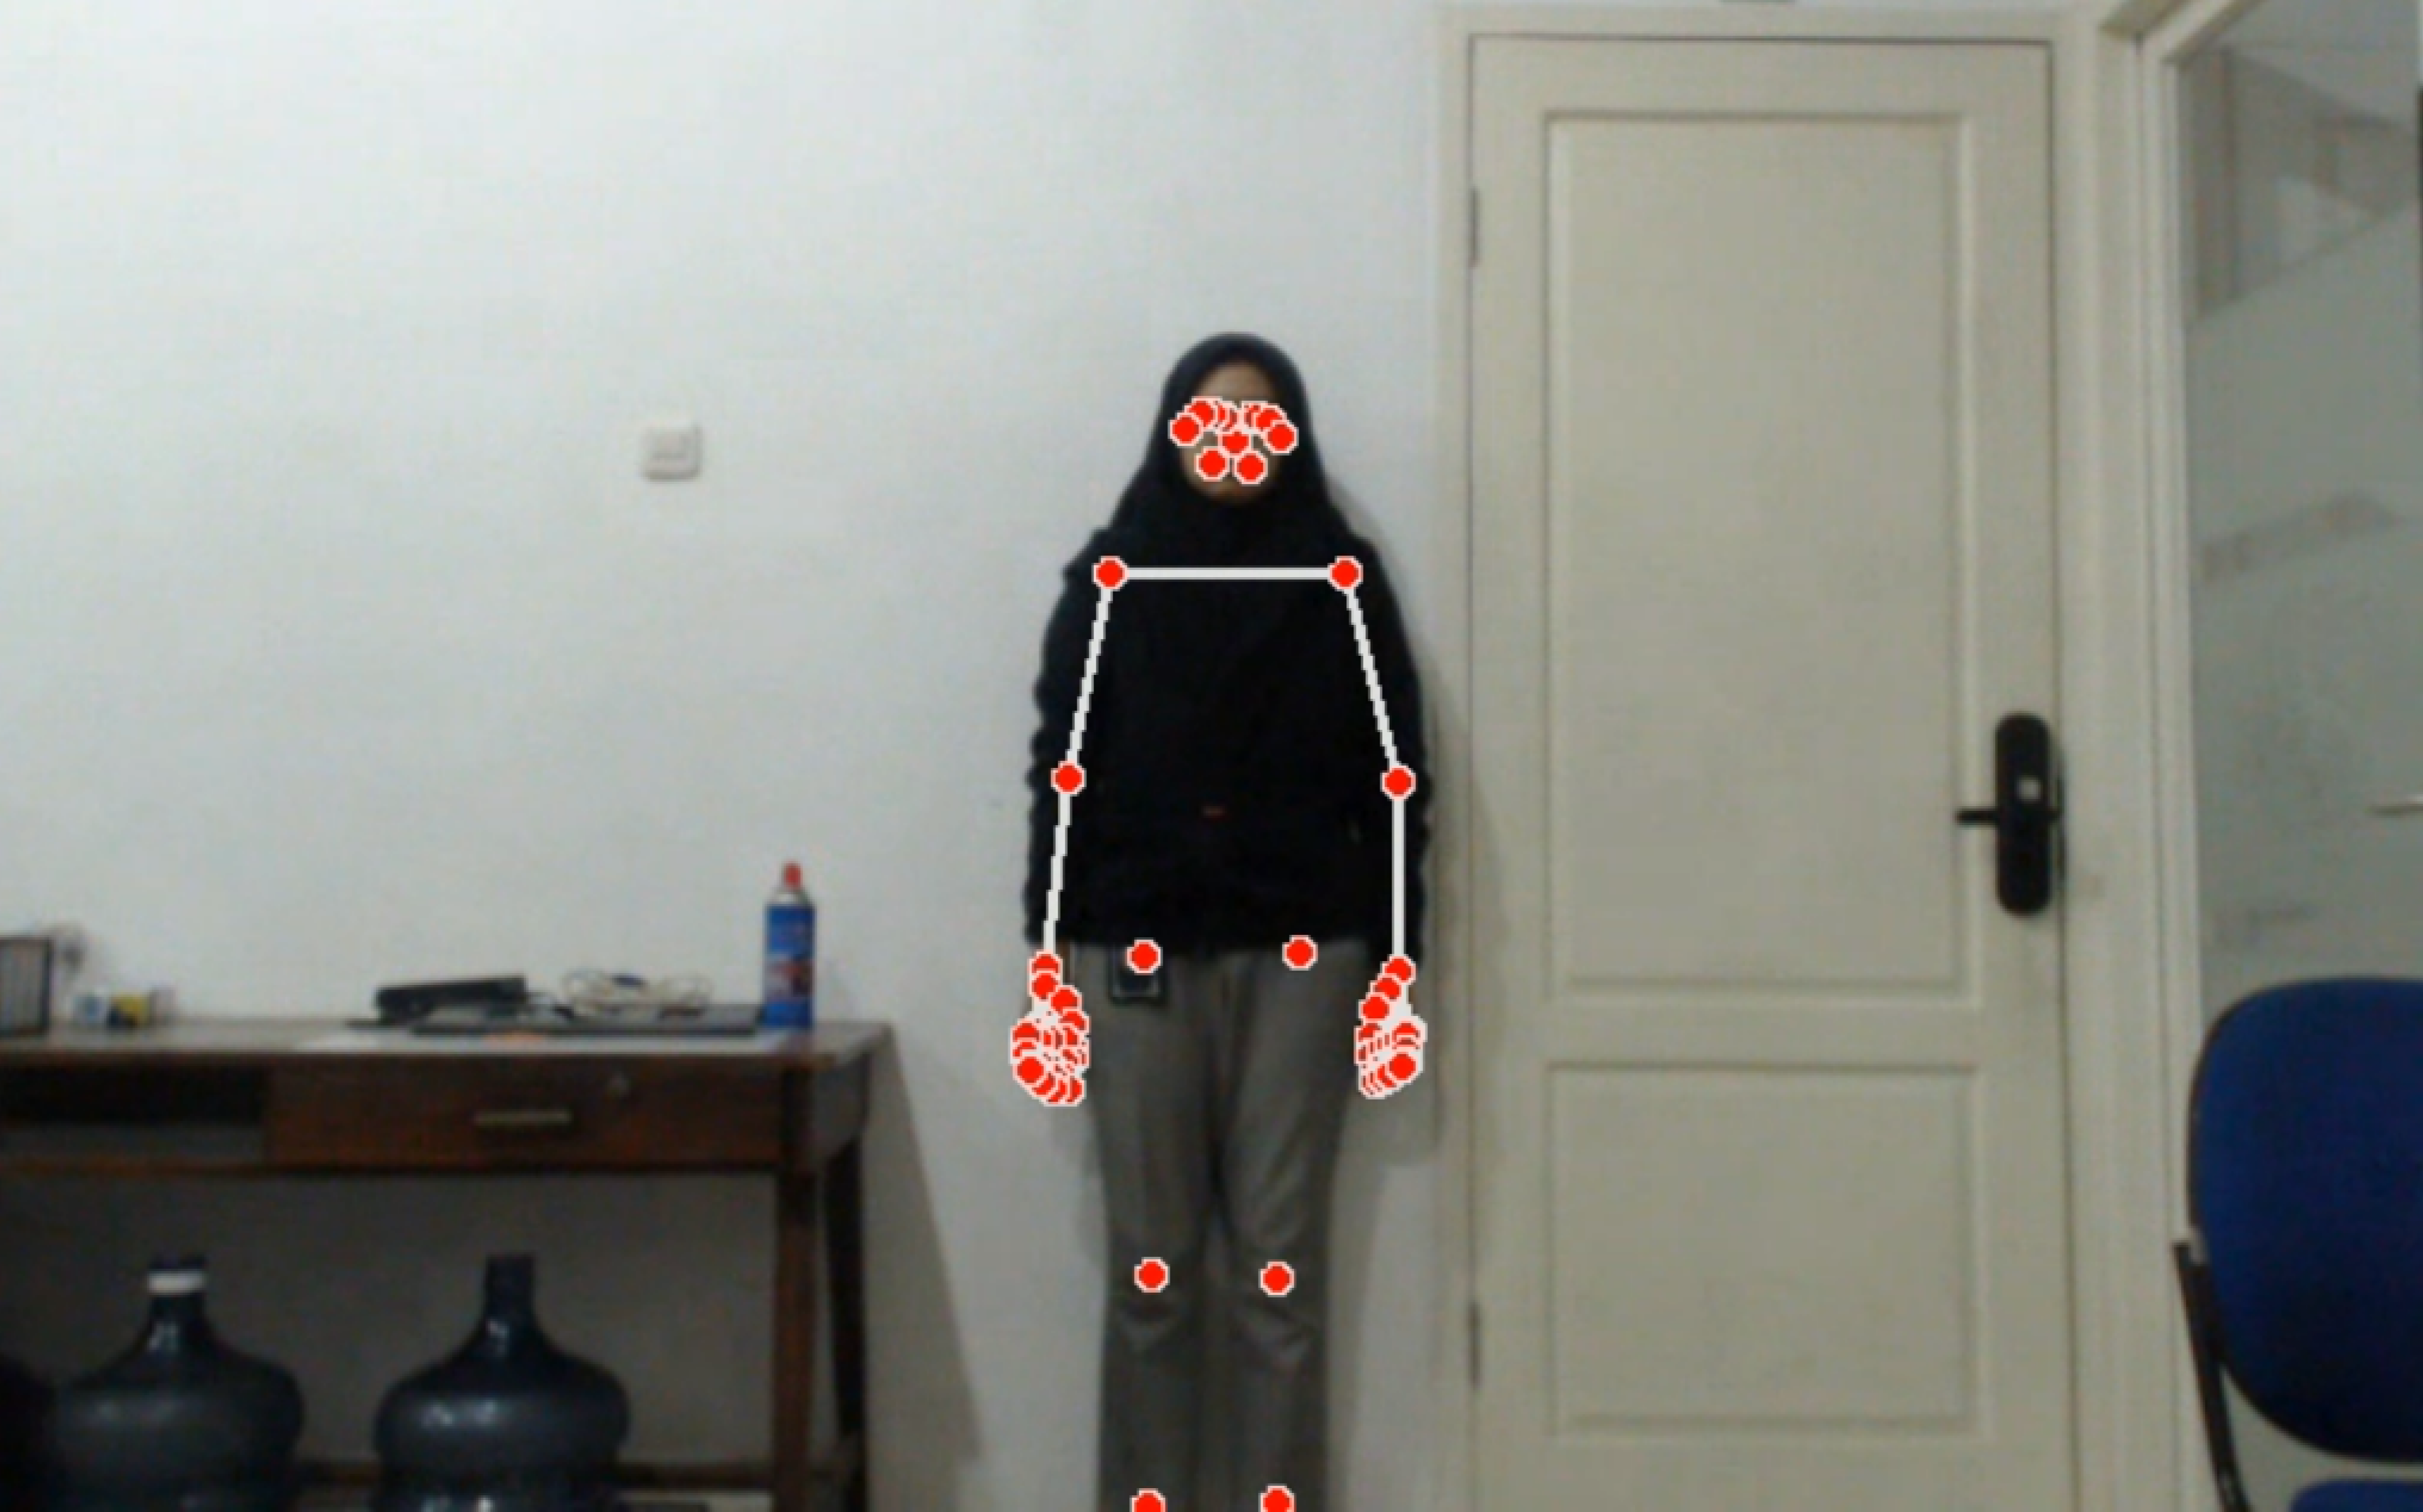
\includegraphics[scale=0.14]{gambar/bab4-rani.png} \\
    \hline
    Male & 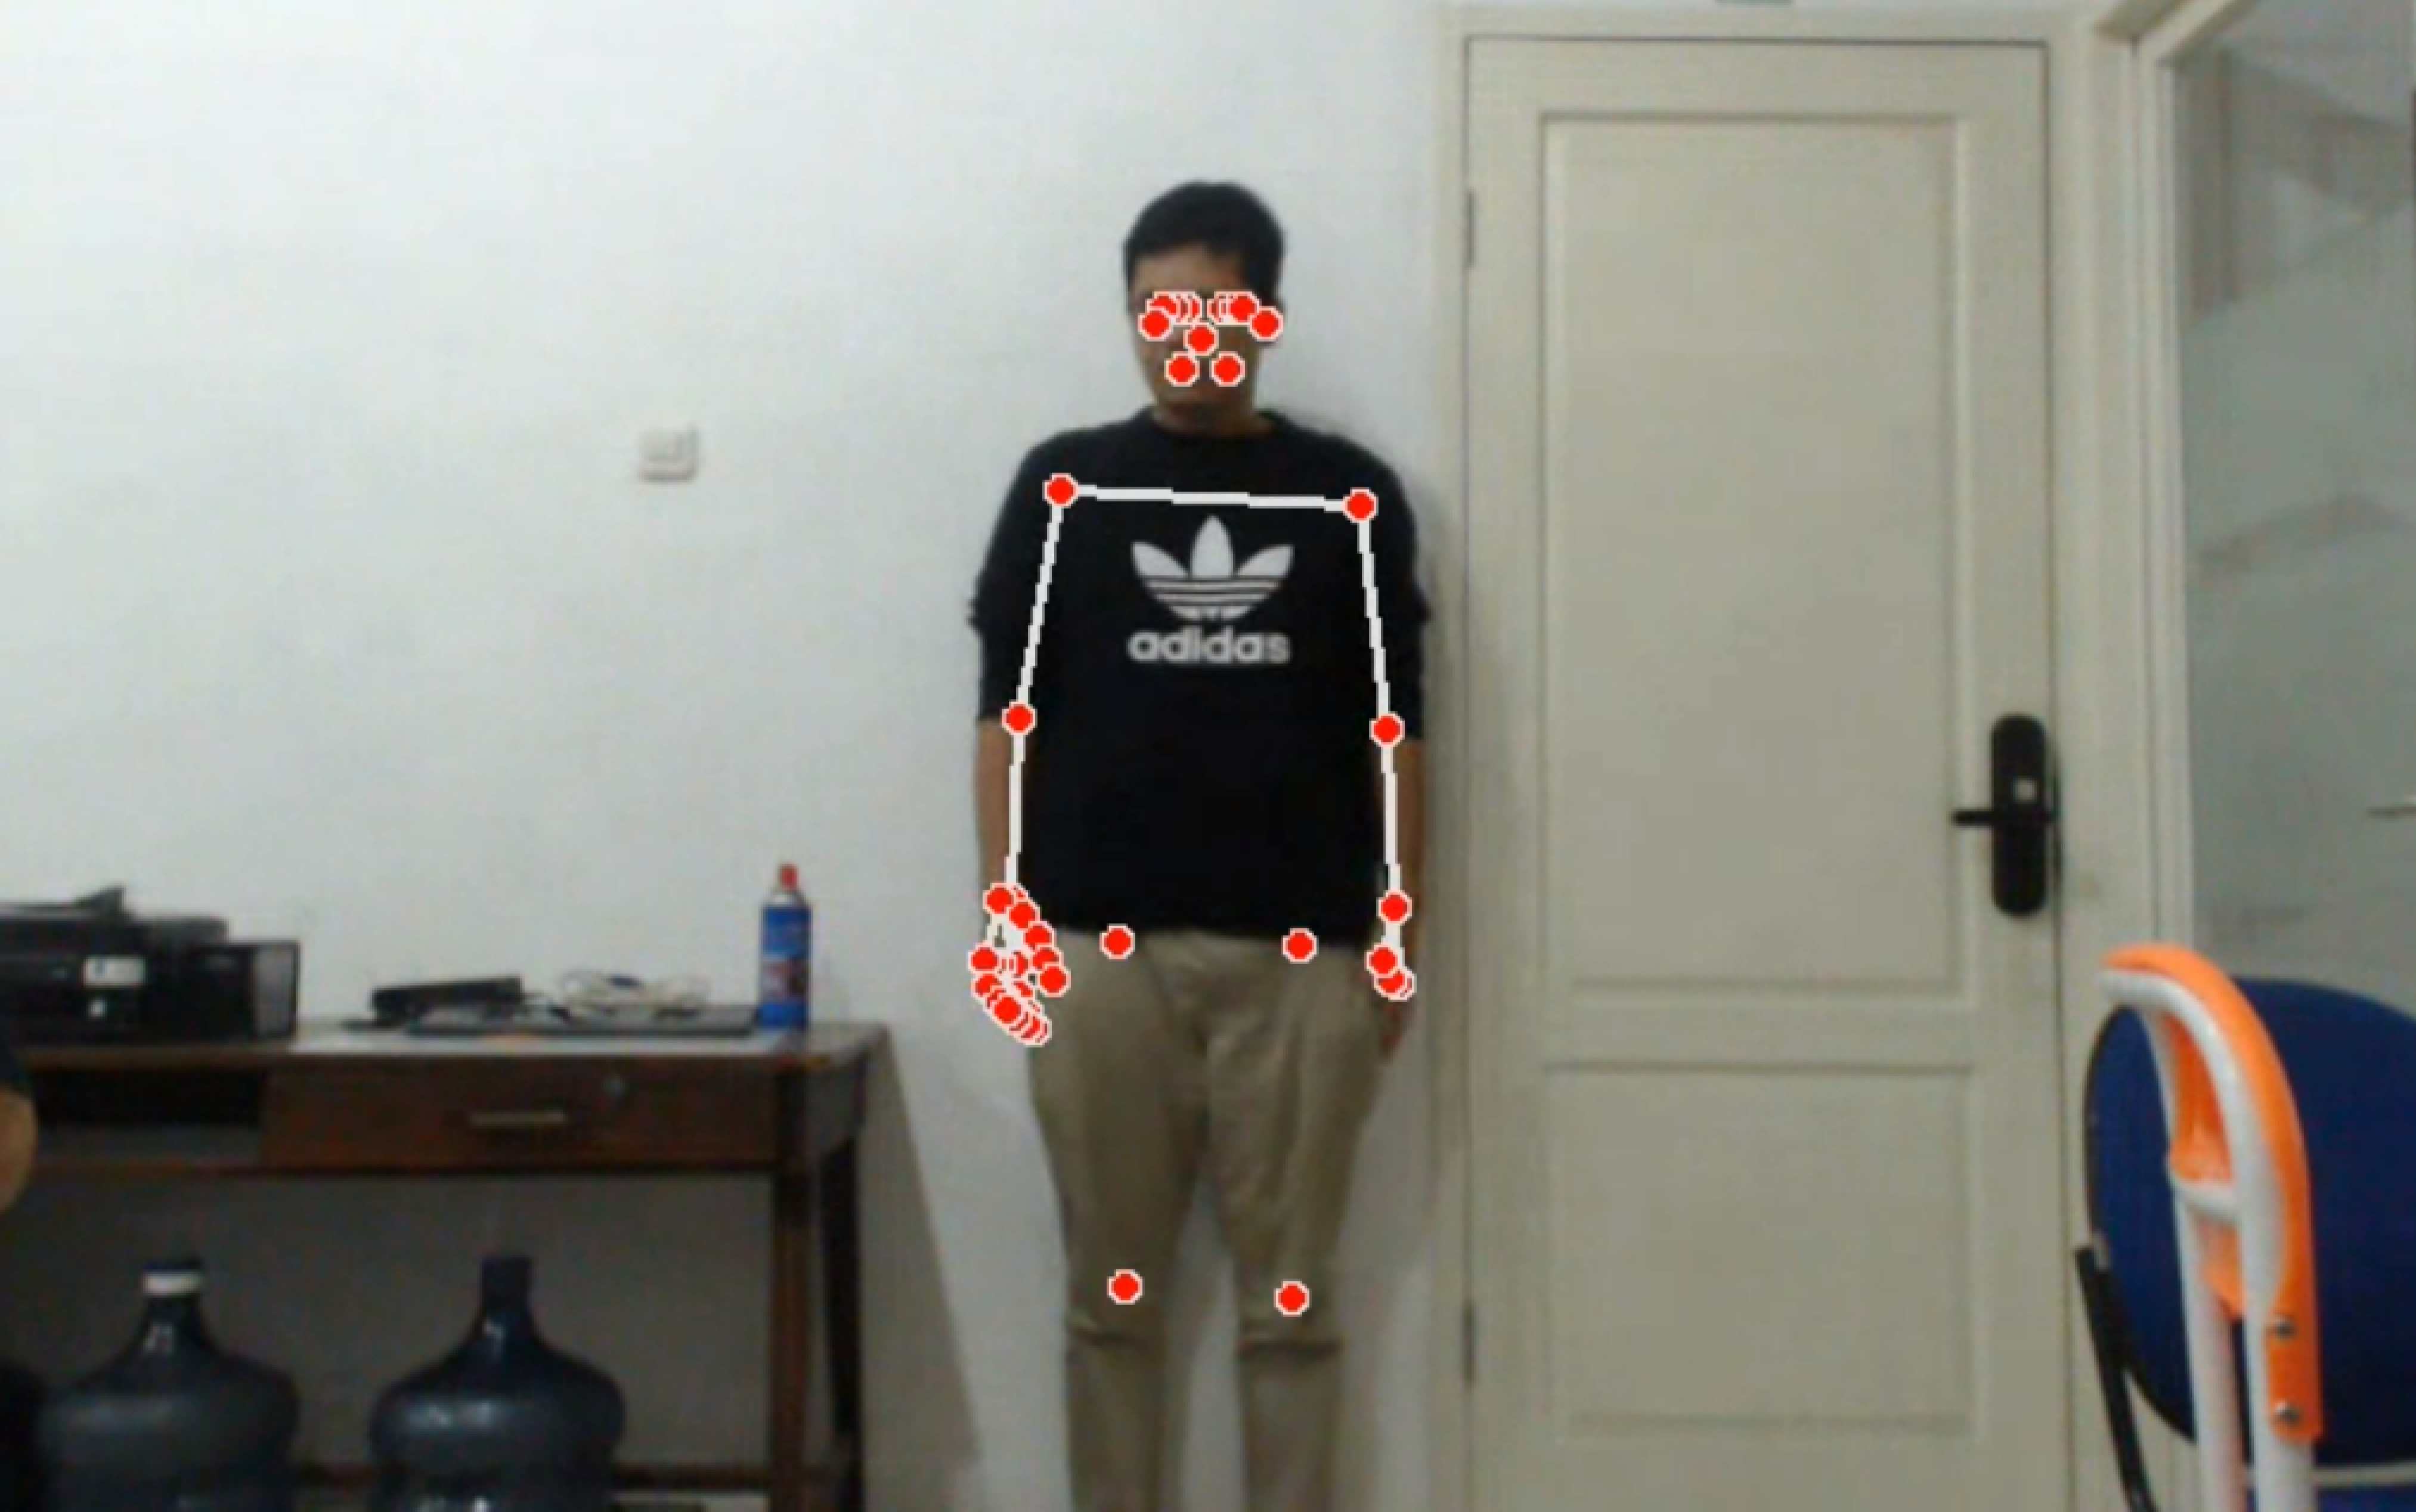
\includegraphics[scale=0.14]{gambar/bab4-evan.png} \\
    \hline
  \end{tabular}
\end{table}

\begin{table}[H]
  \caption{Different Subject Evaluation Results}
  \label{tb:subjectevaluation}
  \centering
  \begin{tabular}{lllll}
    \hline
    \textbf{Subject} & \textbf{Accuracy} & \textbf{Processing Time} & \textbf{Complete Time} & \textbf{FPS}\\
    \hline
    Female & 0.93 & 0.0988 & 2.6636 & 12.026\\
    Male & 0.93 & 0.0973 & 2.8191   & 11.378\\
    \hline
  \end{tabular}
\end{table}

Based on Table \ref{tb:subjectevaluation}, it can be seen that the model can perform classification on different subjects. Data normalization has resulted in a model that is \emph{scale invariant} and \emph{position invariant}. The classification accuracy of the model shows a very good value, which is 0.93 or 93\%. The \emph{average processing time} and \emph{complete time} also show values not far from the tests previously conducted by the author, with the \emph{average processing time} around 0.098 and the \emph{complete time} around 2.74. The average FPS obtained is 11.702. This indicates that the system has good performance in classifying sign movements on different subjects.

\subsection{Sentence Formation and Voice Conversion Testing}
\label{sec:sentenceanalysis}

This test is conducted to understand how the translation system is used to form a series of sentences and perform voice conversion based on the formed sentences. The sentence formation in this system refers to Subsection \ref{subsec:controlsystem}. The sentences will be formed based on a combination of detected vocabulary. The full combination of vocabulary is in Table \ref{tb:vocabularycombination}. This test is performed using the third model tested in Table \ref{tb:modelevaluation}, with a light intensity of 125 lux and a camera distance of 300 cm. A maximum of three repetitions is done for each vocabulary. For each vocabulary combination, control vocabulary is also tested, including "standby," "delete," and "translate."

\begin{table}[H]
  \caption{Vocabulary and Sentence Combinations}
  \label{tb:vocabularycombination}
  \centering
  \begin{tabular}{ll}
    \hline
    \textbf{Vocabulary Combinations} & \textbf{Sentences} \\
    \hline
    "Maaf" + "Siapa" + "Nama" & "Maaf siapa nama kamu?" \\
    "Maaf" + "Tolong" + "Saya" & "Maaf tolong bantu saya" \\
    "Maaf" + "Rumah" + "Siapa" & "Maaf ini rumah siapa?" \\
    "Rumah" + "Saya" & "Ini rumah saya" \\
    "Rumah" + "Siapa" & "Ini rumah siapa?" \\
    "Siapa" + "Nama" & "Siapa nama kamu?" \\
    "Tolong" + "Saya" & "Tolong bantu saya" \\
    \hline
  \end{tabular}
\end{table}

\begin{table}[H]
  \caption{Vocabulary Combination Evaluation Results}
  \label{tb:combinationevaluation}
  \centering
  \begin{tabular}{lllll}
    \hline
    \textbf{Words} & \textbf{Accuracy} & \textbf{Processing Time} & \emph{\textbf{Complete Time}} & \textbf{FPS}\\
    \hline
    2  Words  & 1.00 & 0.0993 & 2.8303 & 13.2573\\
    3  Words  & 0.93 & 0.0981 & 2.0513 & 10.1184\\
    \hline
  \end{tabular}
\end{table}

It can be seen in Table \ref{tb:combinationevaluation} that the model has successfully formed sentences by combining signs sequentially and continuously. This is demonstrated by the accuracy of sentences formed from the combination of 2 words having a value of 1.00 and the combination of 3 words having a value of 0.93. The values of \emph{average processing time} and \emph{average complete time} did not experience significant changes with continuous testing. In the formation of the sentence "Ini rumah saya" ("This is my house"), there was a classification error where the sign for "rumah" ("house") was classified as "delete." This was due to the high similarity between the signs for "rumah" and "delete." Overall, the system's success rate in forming sentences is 0.857 or 85.7\%. The use of the gTTS (Google Text-To-Speech) library has been able to convert the formed sentences well. This is also shown by the successful classification of the "translate" sign in every test conducted. Sentences formed with 3 words tend to have heavier performance compared to 2 words, as indicated by the average FPS values obtained.

Overall, the tests conducted show that the system has good performance in translating a relatively large number of sign movements in \emph{real-time}. The use of the gTTS library has also successfully converted sentences formed by users with an accuracy of up to 100\%.

\begin{figure}[ht]
    \centering
    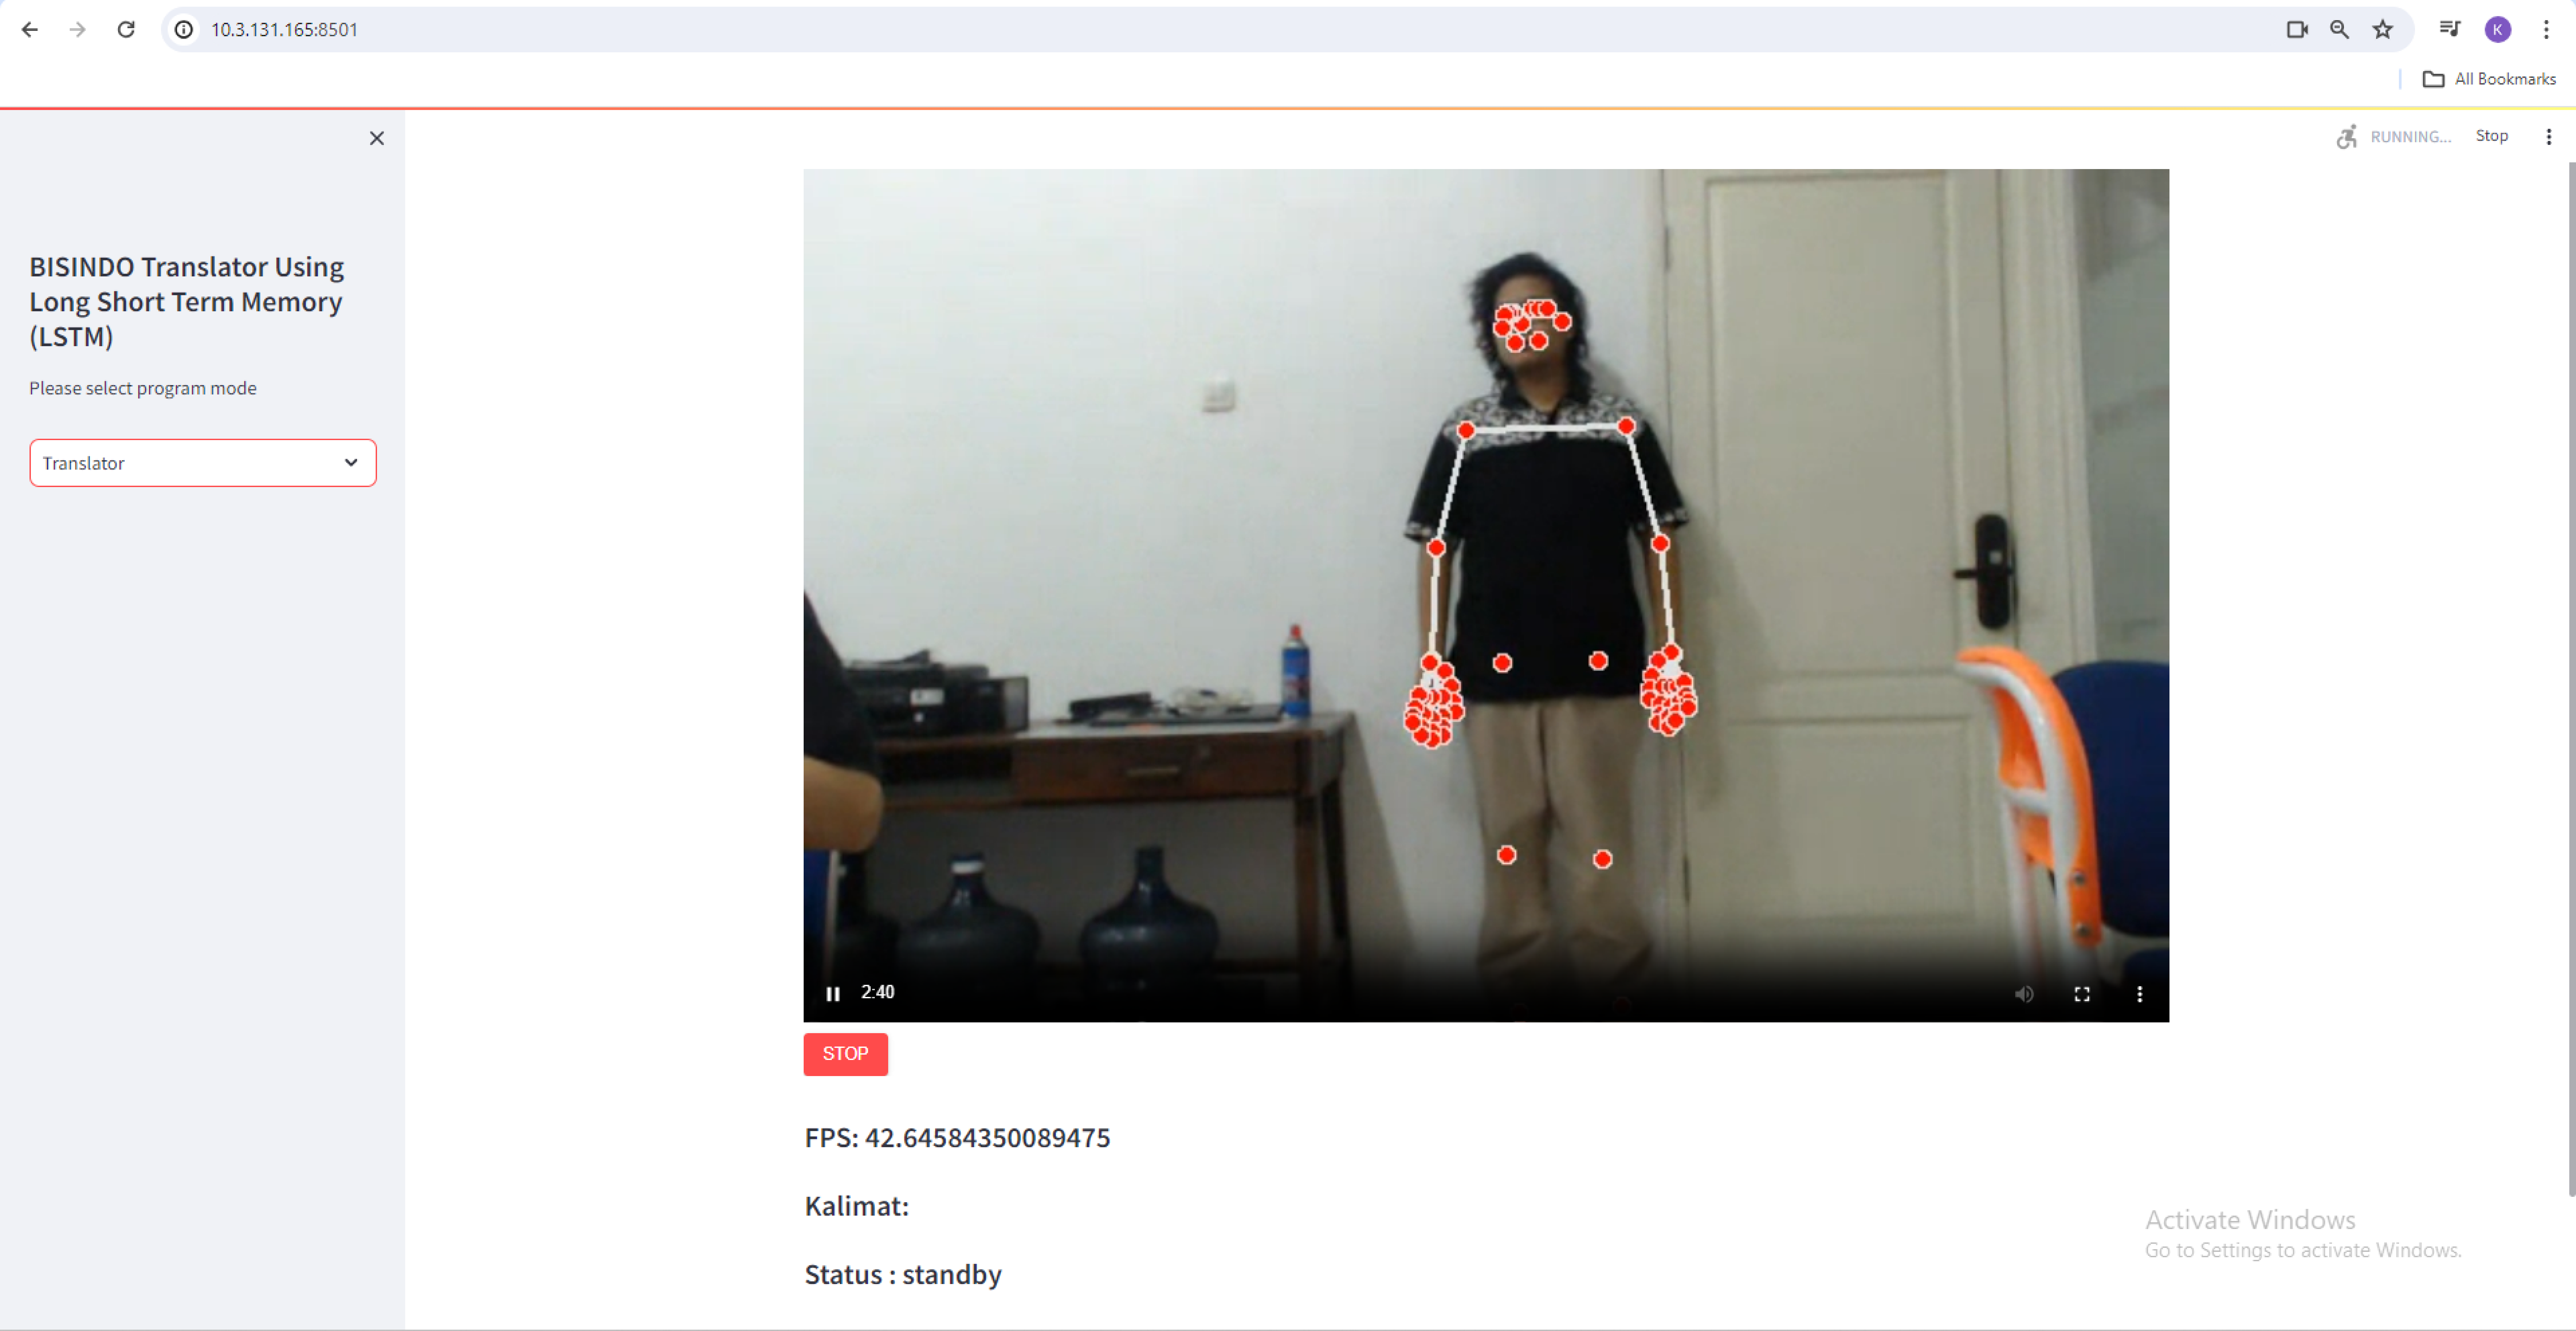
\includegraphics[scale=0.12]{gambar/bab3-layoutweb.png}
    \caption{System Testing Results}
    \label{fig:layoutweb}
\end{figure}
